\section{Introduction}
Suppose an agent is asked: \emph{What was the latest value known by the end of April?} A May release is topically relevant, easy to retrieve, and wrong for the question. On the next period the numbers change, but the required operation does not: filter evidence by the information cutoff. Similar recurring operations arise when an agent must distinguish publication time from reporting time or ground a numerical change in documentary context available at the time. Reusable skills are an appealing way to persist such procedures, but a successful skill run does not by itself identify what was repaired or what part of the implementation deserves credit.

The first problem is the comparator. A targeted helper can beat a generic helper simply because the generic helper degrades the original agent. We observe exactly this pattern on a frozen DeepSeek cutoff cell: targeted T succeeds on 100\%, target-blind G on 72\%, and the original agent N on 100\% of endpoint-repeat observations. A conventional T-versus-G evaluation reports +28 points; adding N changes the verdict to \emph{no repair}. This is not a variance correction. It changes which scientific claim is admissible.

Figure~\ref{fig:e2-scene} turns this identification problem into the running example for the paper. The same cutoff question can make T look beneficial against a mechanism-misaligned stress helper while showing no improvement over the original agent. The lower row previews the next attribution problem: even when net repair exists, helper exposure, targeted operation output, and where that output enters the harness are distinct interventions and need distinct controls.

\begin{figure}[t]
\centering
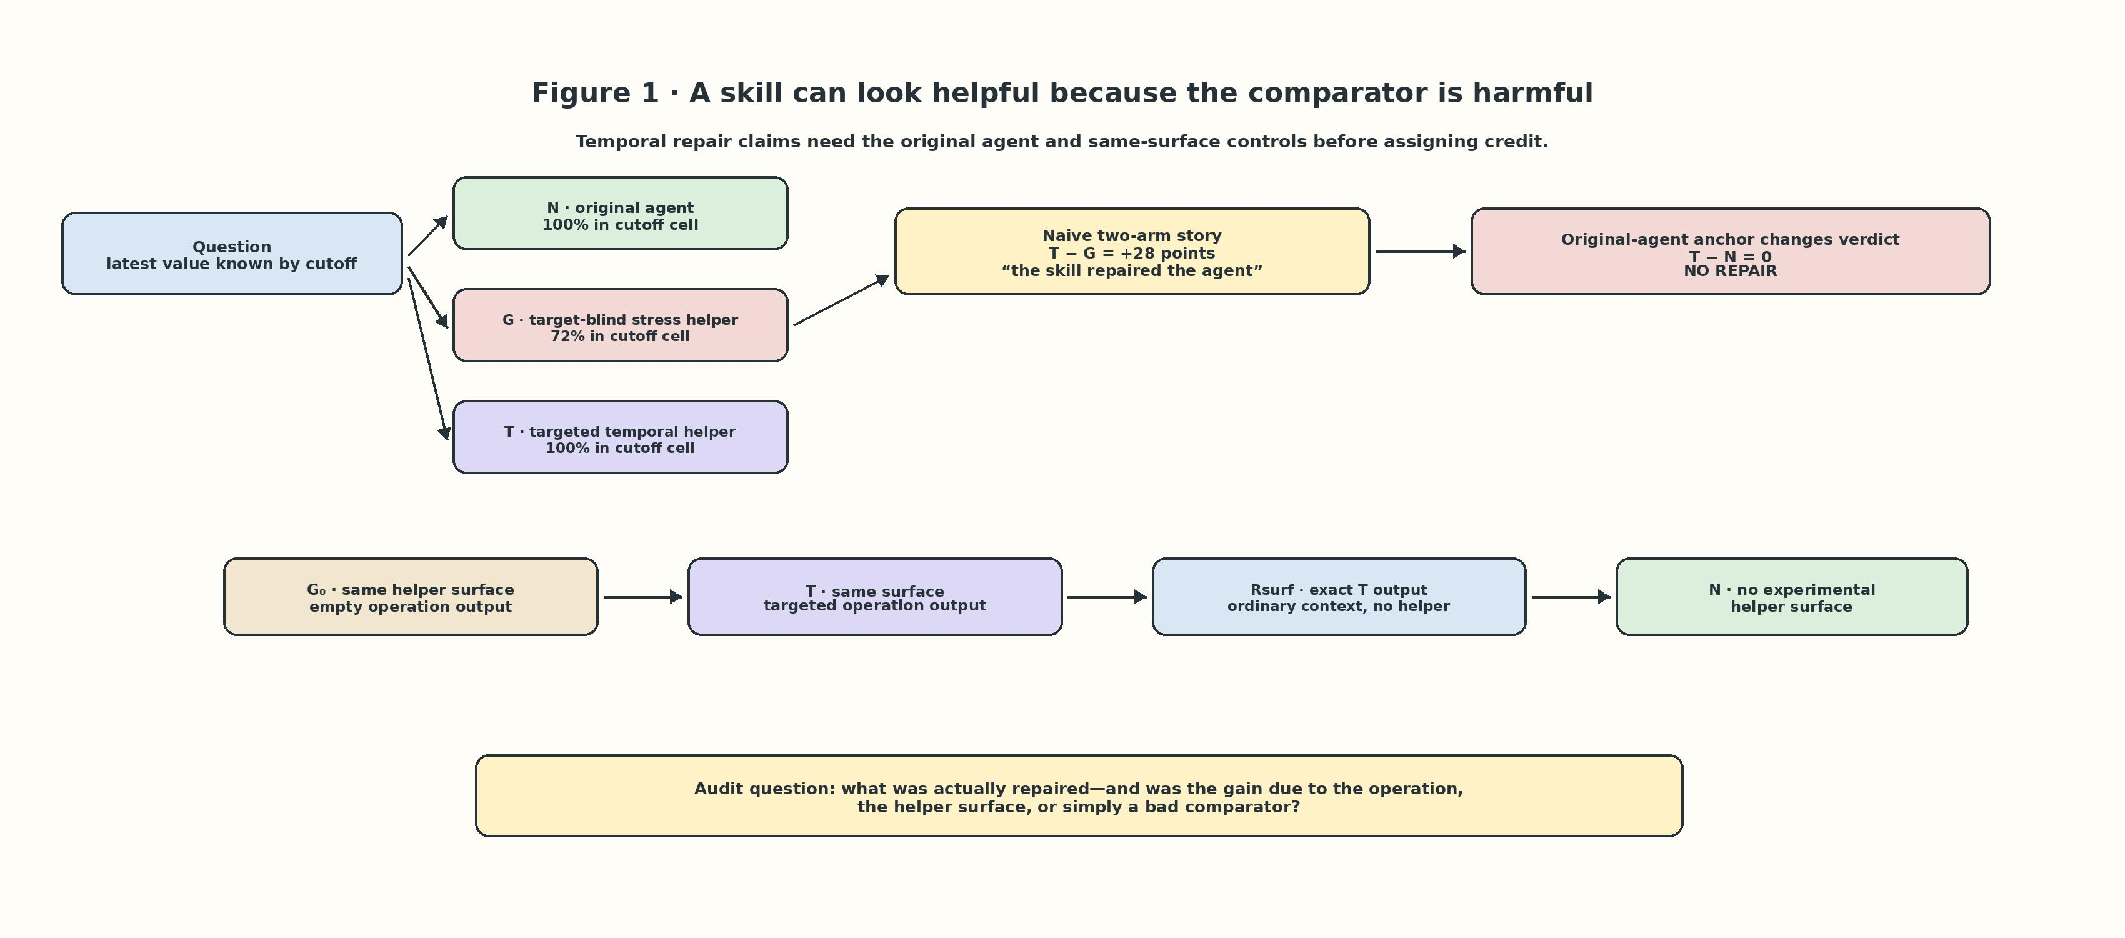
\includegraphics[width=0.99\linewidth]{figures/e2-temporal-repair-scene-handdrawn.pdf}
\caption{\textbf{Scene: a targeted skill can look helpful because its comparator is harmful.} On one frozen DeepSeek cutoff cell, T and the original agent N are both 100\%, whereas the target-blind stress helper G is 72\%. A T-versus-G comparison therefore shows +28 points even though T--N is exactly zero and no repair occurred. The bottom row previews the attribution controls used later: G$_0$ isolates same-surface no-operation exposure, and R$_{\mathrm{surf}}$ holds the exact T output fixed while changing only its integration surface.}
\label{fig:e2-scene}
\end{figure}

The second problem is attribution. We therefore keep four observable contrasts separate:
\begin{equation}
\underbrace{\Delta_{T-N}}_{\text{net repair}},\qquad
\underbrace{\Delta_{T-G_0}}_{\text{same-surface output contrast}},\qquad
\underbrace{\Delta_{G_0-N}}_{\text{surface/placebo perturbation}},\qquad
\underbrace{\Delta_{T-R_{\mathrm{surf}}}}_{\text{integration-surface effect}}.
\end{equation}
G$_0$ is an information-empty no-operation placebo exposed through the same helper surface as T. T--G$_0$ therefore asks whether the targeted operation output changes behavior \emph{conditional on that surface}; G$_0$--N separately reveals whether the surface/placebo itself perturbs the original agent. We do not call T--G$_0$ a pure operation effect when G$_0$--N is nonzero. Algebraically, T--N=(T--G$_0$)+(G$_0$--N), so the three contrasts expose rather than hide a surface interaction. R$_{\mathrm{surf}}$ asks a different question: it runs the identical frozen operation on identical candidate evidence but materializes the exact output in ordinary context instead of callable state. It is deliberately a controlled surface intervention, not an independently learned temporal retriever.

This audit changes several interpretations. Fresh DeepSeek grounding runs have +30 and +20 point T--N and T--G$_0$ directions in C3/C4 with zero observed G$_0$--N shift on those runs, although each cell has only five endpoints. In a post-hoc EIA compatibility probe, T--N is +37.5 points but G$_0$--N is $-25$ points; we use this cell primarily to illustrate net repair with surface interaction, not as confirmation. A Kimi same-domain grounding support cell is downgraded under the fresh controls. The surface audit narrows credit again: across 18 pre-frozen DeepSeek load-bearing endpoints T--R$_{\mathrm{surf}}$ averages 0.0 points. A formal two-one-sided equivalence test at the prospectively frozen $\pm10$-point portfolio margin passes; paired-t and bootstrap 95\% intervals are $[-8.5,8.5]$ and $[-8.3,8.3]$ points, respectively. Because a post-hoc observed-variance sensitivity calculation is only about 53\%, the portfolio is ceiling-heavy, and the strictly non-ceiling subset is too small, we use this only as a low-sensitivity frozen-margin surface check rather than a general equivalence result.

Our setting is a source-native replay built from first-party U.S. Bureau of Economic Analysis (BEA), NOAA Climate Prediction Center, and Energy Information Administration (EIA) release histories~\citep{bea2026archive,noaa2026enso,eia2026wpsrarchive}. The ledger contains 35 frozen endpoints and 2,056 retained runtime-valid rows spanning cutoff validity, release alignment, and exogenous grounding. The initial BEA/NOAA object is motivated by TimeSage-EV but is not an exact rerun because the evaluated TimeSage-EV snapshot remains unavailable~\citep{yao2026timesage}. EIA endpoint construction, the 4/8 temporal split, scorer, procedure hashes, and condition order were frozen before EIA outcomes, but EIA itself was selected post-review because its recurring dated releases are structurally compatible with the cutoff mechanism. We therefore treat it as a post-hoc compatibility probe, not a prospective cross-domain confirmation. Endpoints, not repeated executions, are the independent scientific units.

The paper is an evaluation and identification study, not a skill-learning algorithm. Prior work already studies causal skill attribution, reusable-skill evolution, and temporal retrieval~\citep{zhou2026counterfactual,dong2026agentskills,wang2026notallskills,guan2026continualskillbench,wei2026evoharness,zheng2026skillprox,xu2026hyperskill,asai2024selfrag,yan2024crag,han2025temporalgraphs,wang2026iarag}. We do not claim novelty in procedure reuse, time-aware retrieval, or paired skill causality. The residual contribution is an audit contract for assigning scientific credit and an empirical demonstration that stronger controls can reverse a repair verdict, expose a surface interaction, downgrade a support cell, and erase container-level credit while leaving some net repairs intact.

\paragraph{Contributions.}
We make three contributions. First, we separate net repair, same-surface operation-output contrast, placebo/surface perturbation, and integration-surface effect rather than collapsing them into one ``skill effect.'' Second, we show that this separation changes conclusions: T$>$G but T$=$N is an observed false positive; fresh controls preserve bounded DeepSeek repairs while reclassifying EIA as surface-interacting and downgrading Kimi grounding. Third, an exact-output context-materialization control yields a passing TOST at the prospectively frozen $\pm10$-point \emph{portfolio-average} margin; because the design has low sensitivity and a ceiling-heavy portfolio, we treat this as a frozen-margin surface check while leaving the low-count non-ceiling subset and broader temporal-retrieval questions unresolved. The contribution is therefore methodological understanding: within the registered endpoint portfolio and tested resolution, stronger controls can preserve, narrow, or reverse an apparent reusable-skill effect.

\paragraph{Reader's map.} Figure~\ref{fig:e2-scene} motivates the comparator and attribution problem. Figure~\ref{fig:e2-method} summarizes the full intervention ladder and shows how the later R17 search-projection study fits as a bounded mechanism child rather than a replacement for the R16 paper. The original causal intervention map and regime-effect plot remain as detailed mechanism/result figures.
